\section*{2. Mathematical Framework}

We formalize the recursive dynamics governing quantum state evolution, entropy redistribution, and coherence retention across cosmological cycles. This model is grounded in three principles: \textbf{information flow}, \textbf{thermodynamic asymmetry}, and the \textbf{preservation of structured coherence} via recursive quantum interference.


\subsection*{2.1 Recursive State Evolution and Transition Amplitudes}

We model each cosmological cycle \( n \) as a quantum transition between state vectors \( |\Psi_n\rangle \) and \( |\Psi_{n+1}\rangle \), mediated by a non-unitary, decoherence-weighted evolution operator derived from an effective transition kernel \( K(\phi, \phi') \). This kernel governs the amplitude between field configurations at successive bounces, incorporating discrete quantum geometry, memory filtering, and inherited entanglement structure.

\paragraph{Transition Kernel Definition:}

\begin{equation}
K(\phi,\phi') = \sum_{j_f=0}^{j_{\text{max}}} \prod_f (2j_f+1) \, e^{-j_f(j_f+1)/2j_0^2} \times \exp\left[-\frac{(\Delta\phi - \phi_*)^2}{2\sigma_\phi^2}\right]
\end{equation}

The first term encodes area-quantized contributions from spin-labeled faces in loop quantum gravity. The exponential suppression factor involving \( j_0 \) regulates high-spin fluctuations and is heuristically linked to the minimal ER bridge throat area (see Appendix E.1). The Gaussian envelope in \( \Delta\phi = \phi - \phi' \) acts as a coherence filter, suppressing decoherent transitions and enforcing recursive memory retention. Alternative filtering distributions are discussed in E.1 as well.

\paragraph{Recursive Evolution Law:}

State evolution proceeds via integral recursion:
\begin{equation}
|\Psi_{n+1}\rangle = \int d\phi \, K(\phi, \phi') |\Psi_n(\phi)\rangle
\end{equation}

This evolution reflects a path-integral–like propagation across cycles, where only configurations with high mutual coherence persist. The kernel itself is constructed to favor constructive interference and suppress entropic divergence.

\paragraph{Initial State and Symmetric Structure:}

The recursive configuration inherits information from a symmetric pre-cycle state \( \phi_{U1} \), defined as an interference of left- and right-handed universe branches:
\[
\phi_{U1} = \left\{ p(0),\, p(\pm1),\, p(\pm2),\, \ldots,\, p(\pm n) \right\}
\]
The updated configuration follows a controlled XOR entanglement rule:
\[
\phi_{n+1} = \phi_{U1} \oplus \Psi_n
\]
This XOR operation is formalized in Appendix E.5 as a controlled unitary gate, preserving quantum information while encoding recursive interference.

\paragraph{Recursive Lagrangian Dynamics:}

Each cycle is governed by an effective Lagrangian:
\begin{equation}
\mathcal{L}_n = \frac{1}{2} G_{IJ}(q_n) \dot{q}_n^I \dot{q}_n^J - V(q_n) + D[\rho_n] - M_n(q_n, q_{n-1}) + \mathcal{F}_{\text{ERB}}
\end{equation}
Where:
\begin{itemize}
  \item \( G_{IJ} \): Field-space metric from LQC geometry.
  \item \( D[\rho_n] \): Non-Markovian decoherence functional (see Section 2.4, Appendix E.2).
  \item \( M_n \): Memory interaction term coupling prior cycles.
  \item \( \mathcal{F}_{\text{ERB}} \): Coherence-carrying Einstein–Rosen bridge functional (see Section 2.3, Appendix E.3).
\end{itemize}

This Lagrangian underlies the recursive attractor convergence mechanism and encodes both local field dynamics and cross-cycle memory propagation.

\paragraph{Summary:}

This section formalizes the recursive evolution of quantum states in a cyclic cosmological model. The transition kernel selectively favors low-entropy, memory-preserving paths; the entangled XOR composition of configurations ensures recursive inheritance of structure; and the effective Lagrangian provides a dynamical backbone for attractor formation. Detailed derivations and justifications for each component are provided in Appendix E.
\subsection*{2.2 The Transition Kernel as a Coherence Filter}

The transition kernel \( K(\phi, \phi') \) serves as the central structure through which quantum information propagates across cosmological bounces. In our framework, this kernel enforces both geometric discreteness and memory coherence, acting as a selective filter that probabilistically favors consistent, low-entropy transitions.

\paragraph{Semiclassical Approximation:}

In the semiclassical regime—where quantum geometry effects remain significant but spacetime curvature is below Planckian scales—the kernel admits an approximate path-integral form:
\begin{equation}
K(\phi, \phi') \approx \exp\left[i \int_{\Sigma} \left(\pi^a \dot{\phi}_a - H_{\text{eff}}(\phi, \phi')\right) \, d^3x\right]
\end{equation}
Here, \( \Sigma \) is the bounce hypersurface, and \( H_{\text{eff}} \) includes holonomy and inverse-volume corrections typical of Loop Quantum Cosmology (LQC)~\cite{ashtekar2006quantum}. The path integral is dominated by coherent histories aligned with saddle points of the action, favoring configurations that preserve phase and entanglement across bounces.

\paragraph{Coherence Filtering Envelope:}

The Gaussian in the heuristic form of the kernel (see Eq.~(1)) acts as a memory filter:
\[
\exp\left[-\frac{(\Delta\phi - \phi_*)^2}{2\sigma_\phi^2}\right]
\]
This term suppresses destructive interference and favors pointer states—stable field configurations resilient to decoherence. The filter preserves recursive memory while minimizing entropy production, inspired by quantum Darwinism~\cite{zurek2003decoherence}.

\paragraph{Generalized Filter Structures:}

While the Gaussian filter captures coherent evolution under mild fluctuation, it may not capture rare, high-impact deviations that seed new structure. In Appendix E.1, we propose replacing this with a Lévy-stable distribution:
\[
\exp\left[-\frac{|\Delta\phi - \phi_*|^\alpha}{2\sigma^\alpha}\right], \quad 0 < \alpha < 2
\]
Such heavy-tailed filters allow for sporadic large jumps, modeling intermittent coherence surges and rare tunneling-like events across field space.

\paragraph{Microscopic Interpretation from LQG:}

The spin-sum component of the kernel:
\[
\sum_{j_f} \prod_f (2j_f + 1) e^{-j_f(j_f+1)/2j_0^2}
\]
is justified in Appendix E.1 as arising from EPRL spinfoam amplitudes in the large-spin limit, where vertex amplitudes asymptote to the Regge action and the prefactor regulates semiclassical saddle-point suppression. The dominant spin \( j_0 \) is tied to the area of the Einstein–Rosen bridge throat and constrains the effective memory channel size.

\paragraph{Summary:}

The transition kernel filters and weights the propagation of quantum field configurations across cosmological cycles. It is structured to reinforce coherent memory retention while suppressing entropic or decoherent transitions. The kernel thus plays a dual role as a dynamical propagator and a thermodynamic selector, enabling the emergence of attractors and long-range recursive order. For a complete derivation and proposed refinements, see Appendix E.1.

\subsection*{2.3 Einstein–Rosen Bridge as Coherence Channel}

The Einstein–Rosen bridge (ERB), rather than being a traversable wormhole, is treated in our model as an entanglement-preserving geometric structure that transmits partial quantum information across cosmological bounces. This bridge provides a continuity channel constrained by both geometric entropy bounds and mutual information fidelity.

\paragraph{Action Structure of the ERB:}

We define the ERB contribution to the total action as:
\begin{equation}
S_{\text{ERB}}(\phi, \phi') = \frac{A(\phi, \phi')}{4G\hbar} + i \lambda_E I(\phi, \phi')
\end{equation}
Here:
\begin{itemize}
    \item \( A(\phi, \phi') \) is the minimal area of the bridge throat connecting field configurations \( \phi \) and \( \phi' \),
    \item \( I(\phi, \phi') \) is the mutual information between these configurations, quantifying coherence transmission,
    \item \( \lambda_E \) is a cycle-dependent coherence coupling constant inherited from the previous recursive update.
\end{itemize}

The real part governs the entropic cost of maintaining connectivity, while the imaginary part modulates phase coherence and appears in the transition kernel as a complex weight.

\paragraph{Unitarity and Coherence Preservation:}

The imaginary contribution \( i \lambda_E I(\phi, \phi') \) does not violate unitarity in the path-integral formulation. Rather, it reflects selective reinforcement of entangled histories—favoring transitions that maximize memory continuity while obeying boundary entropy constraints:
\[
S_{\text{rec}}(\phi') \leq \frac{A(\phi, \phi')}{4G\hbar}
\]
This inequality, derived from the Quantum Focusing Conjecture and quantum extremal surface theorems~\cite{engelhardt2015coarse, almheiri2019entropy}, guarantees that recoverable information remains bounded by geometric capacity.

\paragraph{Spin Network Realization:}

In Loop Quantum Gravity, the area term derives from the spin-network puncture representation:
\[
A(\phi, \phi') = 8\pi \gamma \ell_P^2 \sum_f \sqrt{j_f(j_f+1)}
\]
This connects the ERB geometry directly to the spin-sum structure in the transition kernel \( K(\phi, \phi') \), establishing internal consistency between geometric quantization and coherence dynamics.

\paragraph{Mutual Information as Recursive Memory:}

The mutual information \( I(\phi, \phi') \) quantifies the degree of structure preserved across the bounce. As shown in Appendix E.3, the recursive coherence strength \( \lambda_E \) evolves with the fidelity of prior states:
\[
\lambda_E \sim -\log \left( |\langle \Psi_{n-1} | \Psi_n \rangle|^2 + \epsilon \right)
\]
This coupling penalizes incoherent transitions and enhances memory reinforcement, effectively controlling the throughput of the ERB channel.

\paragraph{Energy Interpretation:}

The ERB action contributes to the total energy budget per cycle, as detailed in Section 2.6. The term \( T_H \Delta S_{\text{holo}} \) arises from Brown-York quasi-local energy flux through the bridge and is proportional to its minimal area. This embeds thermodynamic consistency directly into the recursive framework.

\paragraph{Summary:}

The ERB acts as a bounded, coherence-weighted memory conduit across cosmological cycles. Its area constrains entropic throughput, while mutual information modulates quantum fidelity. This duality—between geometry and coherence—enables partial self-remembering in the evolution of the universe, offering a physically motivated mechanism for recursive information propagation. For derivation and first-principles justification, see Appendix E.3.

\subsection*{2.4 Non-Markovian Decoherence with Memory}

To capture coherence decay and information loss within each cosmological cycle, we employ a non-Markovian master equation with memory effects. This approach allows quantum decoherence to be influenced by prior states, consistent with the recursive dynamics of the Self-Remembering Universe.

\paragraph{Master Equation:}

The evolution of the reduced density matrix \( \rho(t) \) follows:
\begin{equation}
\dot{\rho}(t) = -\frac{i}{\hbar}[H, \rho(t)] + \int_0^t D(\tau) [O, [O, \rho(t - \tau)]] \, d\tau
\end{equation}
where:
\begin{itemize}
    \item \( H \) is the effective Hamiltonian governing coarse-grained cosmological degrees of freedom,
    \item \( O \) is the observable coupling to environmental modes (e.g., horizon-crossing modes),
    \item \( D(\tau) \) is a memory kernel encoding time-nonlocal coherence decay.
\end{itemize}

\paragraph{Memory Kernel Form:}

We assume an oscillatory damping form:
\begin{equation}
D(\tau) = \gamma(E) \, e^{-\tau / \tau_c(E)} \cos(\omega_0 \tau)
\end{equation}
Here:
\begin{itemize}
    \item \( \gamma(E) \) is an energy-dependent decoherence strength,
    \item \( \tau_c(E) \) is the coherence time, potentially tied to Planck-scale physics,
    \item \( \omega_0 \) is the memory oscillation frequency (e.g., dominant field resonance).
\end{itemize}

This kernel reflects two key features:
\begin{enumerate}
    \item \textit{Exponential decay} consistent with thermodynamic irreversibility,
    \item \textit{Oscillatory structure} enabling periodic re-coherence events near bounces.
\end{enumerate}

\paragraph{Recursive Role:}

The memory kernel directly shapes the overlap \( \langle \Psi_n | \Psi_{n+1} \rangle \), regulating the degree of fidelity propagation. As shown in Section 2.5 and Appendix E.2, this overlap controls recursive entropy and the effectiveness of ERB coherence transmission. In the Markovian limit (\( \tau_c \to 0 \)), memory is lost completely; in the high-coherence limit (\( \tau_c \gg \Delta t_{\text{cycle}} \)), attractor behavior can emerge.

\paragraph{Observer Dependence and Operator Context:}

The observable \( O \) may represent horizon flux, curvature operators, or entanglement-sensitive modes. Because decoherence depends on observer partitioning of information, \( O \) encodes the contextual interface between subsystems (e.g., internal vs. boundary).

\paragraph{Visualization:}

\begin{figure}[H]
\centering
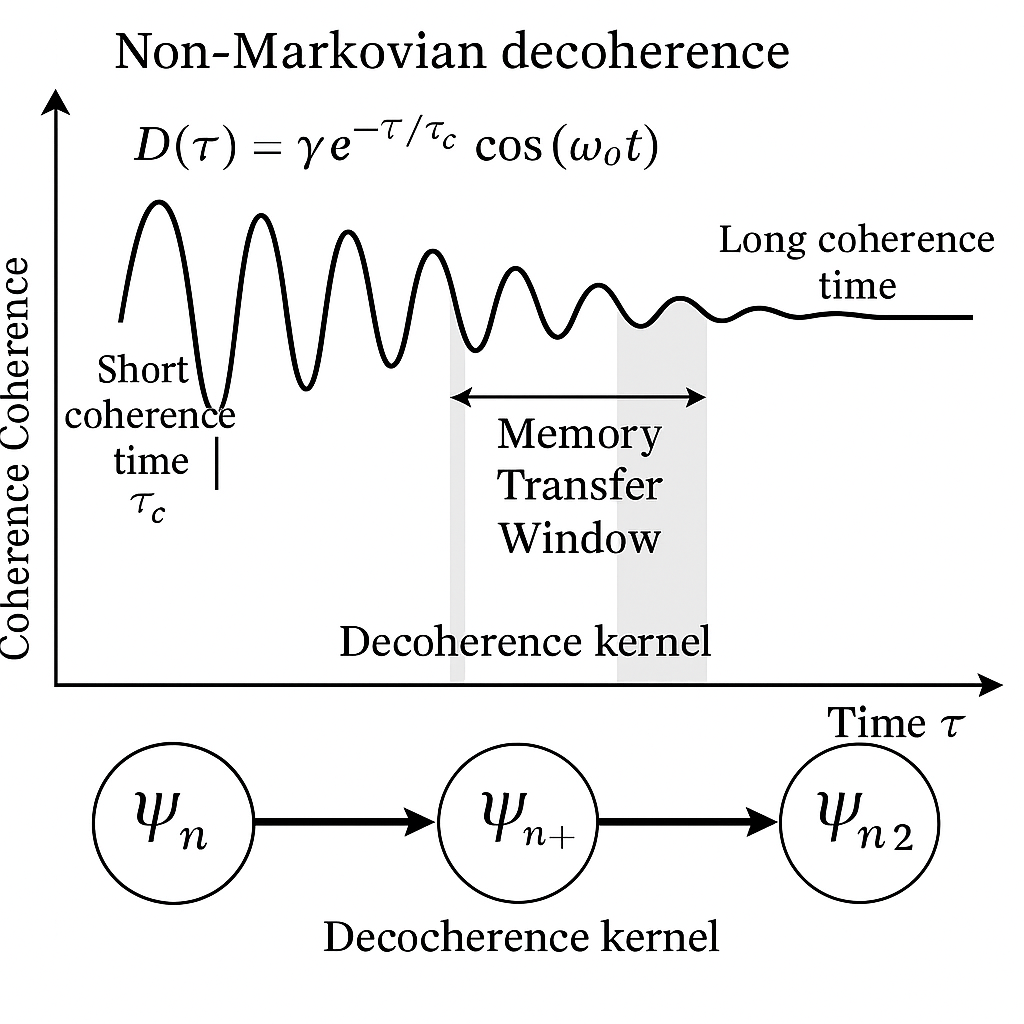
\includegraphics[width=0.72\textwidth]{figures/non_markovian_memory_kernel.png}
\caption{Illustration of the memory kernel \( D(\tau) = \gamma \, e^{-\tau/\tau_c} \cos(\omega_0 \tau) \). The oscillatory decay structure models partial coherence preservation with periodic re-coherence, enabling memory transmission across cosmological cycles.}
\label{fig:memory_kernel}
\end{figure}

\paragraph{Summary:}

Non-Markovian decoherence provides the core mechanism for modeling partial memory retention and coherence filtering in recursive cosmology. The kernel \( D(\tau) \), shaped by energy and timescale parameters, defines how much of the quantum past survives into the next cycle. This structure bridges entropy dynamics, ERB memory throughput, and the emergence of attractor states. For mathematical resolution and microscopic justification, see Appendix E.4.

\subsection*{2.5 Recursive Entropy and Holographic Continuity}

Entropy across cycles is governed by both geometric area and quantum coherence. The recursive entropy functional reflects a hybrid of holographic geometry and overlap fidelity between quantum states of successive cycles.

\paragraph{Baseline Formulation:}

We begin with the regularized coherence-weighted entropy:

\begin{equation}
S_n = \frac{A_{n-1}}{4G\hbar} - \lambda_S \log \left( |\langle \Psi_{n-1} | \Psi_n \rangle|^2 + \epsilon \right)
\end{equation}

\noindent
where:
\begin{itemize}
    \item \( A_{n-1} \) is the minimal-area bounding surface of the prior cycle (e.g., ERB throat),
    \item \( \lambda_S \) is a coherence-entropy coupling constant,
    \item \( \epsilon \ll 1 \) is a regulator to ensure finiteness for orthogonal states.
\end{itemize}

This expression accounts for:
\begin{enumerate}
    \item Geometric entropy inherited from loop quantum gravity’s Bekenstein-Hawking area law,
    \item Memory degradation due to decoherence, captured by decreasing overlap fidelity.
\end{enumerate}

\paragraph{Resolution of Divergence:}

To address divergences when \( \langle \Psi_{n-1} | \Psi_n \rangle \to 0 \), we adopt the quantum relative entropy between reduced states \( \rho_n, \rho_{n-1} \):

\begin{equation}
S_n = \frac{A_{n-1}}{4G\hbar} + \lambda_S \, \text{Tr}[\rho_n (\log \rho_n - \log \rho_{n-1})]
\end{equation}

This form:
\begin{itemize}
    \item Remains finite even for orthogonal states,
    \item Encodes both classical and quantum distinguishability,
    \item Ensures monotonic growth under completely positive trace-preserving (CPTP) maps.
\end{itemize}

\paragraph{Recursive Inequality:}

We impose the entropy bound:

\begin{equation}
S_{n+1} \leq S_n - S_{\text{BH}} + \Delta S_{\text{holo}}
\end{equation}

where:
\begin{itemize}
    \item \( S_{\text{BH}} \): Entropy sequestered in black holes during cycle \( n \),
    \item \( \Delta S_{\text{holo}} \): Holographically recoverable entropy transferred via the ER bridge.
\end{itemize}

This inequality ensures causal consistency and bounds the memory propagation within holographic limits.

\paragraph{Holographic Context:}

From the ERB perspective, entropy recovery is constrained by the Ryu-Takayanagi (RT) bound:

\[
S_{\text{rec}}(\phi') \leq \frac{A(\phi, \phi')}{4G\hbar}
\]

which matches the leading term in the recursive entropy expression. The ERB channel thus functions as a bounded entropy conduit that transfers recoverable structure across bounces.

\paragraph{Entropy as Memory Proxy:}

The quantum relative entropy between \( \rho_n \) and \( \rho_{n-1} \) quantifies the memory drift between cycles. High coherence implies \( \rho_n \approx \rho_{n-1} \), minimizing entropy production and preserving structure. In the attractor regime (see §2.7), this overlap stabilizes and entropy saturates.

\paragraph{Summary:}

Recursive entropy unifies holographic geometry with quantum information fidelity. The relative entropy regularization enforces continuity even in the presence of orthogonal transitions and provides a robust formalism for modeling entropy flow in cyclic cosmology. For further refinement and open issues, see Appendix E.2.

\subsection*{2.6 Energy Transfer Across Cycles}

Energy transfer between cosmological cycles is mediated by the Einstein–Rosen bridge (ERB), which encodes both geometrical and quantum informational continuity. We propose a quasi-local thermodynamic model that links energy flux to entropy flow across the bounce surface.

\paragraph{Phenomenological Energy Balance:}

We define the inter-cycle energy change as:

\begin{equation}
\Delta E_n \approx T_H \Delta S_{\text{holo}} + Q_{\text{ERB}} - \lambda_E I(\phi, \phi')
\end{equation}

\noindent
with:
\begin{itemize}
    \item \( T_H \): Effective Hawking–Unruh-like temperature at the ERB throat,
    \item \( \Delta S_{\text{holo}} \): Holographically transferable entropy across the bridge,
    \item \( Q_{\text{ERB}} \): Quasi-local energy from ERB fluctuations (e.g., quasinormal modes, area variance),
    \item \( \lambda_E I(\phi, \phi') \): Coherence cost due to mutual information divergence between cycles.
\end{itemize}

This reflects a balance between geometric transmission, quantum interference constraints, and thermodynamic irreversibility.

\paragraph{Quasi-Local Derivation:}

To ground the heuristic in gravitational thermodynamics, we invoke the Brown–York tensor at the bridge surface \( S \):

\begin{equation}
E_{\text{BY}} = \int_S d^2x \sqrt{\sigma} \, T^{ab}_{\text{BY}} u_a \xi_b
\end{equation}

where:
\begin{itemize}
    \item \( \sigma \): Determinant of the induced 2-metric on \( S \),
    \item \( T^{ab}_{\text{BY}} \): Brown–York stress-energy tensor derived from extrinsic curvature,
    \item \( u^a \): Normal vector to \( S \),
    \item \( \xi^a \): Timelike Killing vector generating bridge evolution.
\end{itemize}

The energy flux across cycles then becomes:

\begin{equation}
\Delta E = \frac{\kappa \Delta A}{8\pi G} + \text{(work terms)}
\end{equation}

with \( \kappa \) the surface gravity and \( \Delta A \) the area change of the ERB throat.

\paragraph{Holographic Bound:}

The energy transmissible through the ERB is bounded by the bridge’s holographic capacity:

\begin{equation}
\Delta E_{\text{bridge}} \leq \frac{A_{\text{ERB}}}{4G} \cdot T_H
\end{equation}

This matches the form expected from the AdS/CFT-inspired relation between energy and entropy bounds in a bulk-bounded channel.

\paragraph{Coherence Penalty:}

The coherence term \( \lambda_E I(\phi, \phi') \) functions as a backreaction penalty on information-rich transitions. When cycles become highly dissimilar (i.e., mutual information drops), the coherence cost increases, reducing net energy transfer efficiency.

This mechanism suppresses energetically disruptive transitions and enforces smoother evolution across the cyclic chain. It parallels dissipative terms in nonequilibrium thermodynamics and ensures that only phase-aligned, entanglement-preserving states dominate in long-term evolution.

\paragraph{Recursive Energy Conservation:}

The recursion rule for energy across cycles becomes:

\begin{equation}
E_{n+1} = E_n - \Delta E_{\text{diss}} + \Delta E_{\text{bridge}}
\end{equation}

where \( \Delta E_{\text{diss}} \) includes energy lost to black hole evaporation, radiation, and decoherence noise within the cycle.

\paragraph{Summary:}

Energy transmission in this framework is a geometric–informational process governed by quasi-local gravitational flux, bounded entropy flow, and coherence-weighted penalties. The Einstein–Rosen bridge acts as both a thermodynamic interface and a filter for memory-compatible energy transfer. For derivation details and future directions, see Appendix E.3.

\subsection*{2.7 Fixed-Point Attractor Dynamics}

A central prediction of the recursive quantum cosmology model is the emergence of a stable fixed-point attractor state \( \Psi^*(\phi) \) in Hilbert space. This state represents a limit of recursive convergence, where the quantum memory field saturates in coherence and structure across cosmological cycles.

\paragraph{Definition and Properties:}

We define the attractor via recursive convergence:

\begin{equation}
\lim_{n \to -\infty} \Psi_n(\phi) = \Psi^*(\phi)
\end{equation}

This implies \( \Psi^*(\phi) \) satisfies the fixed-point equation:

\begin{equation}
\int K(\phi, \phi') \Psi^*(\phi') \, d\phi' = \Lambda \Psi^*(\phi)
\end{equation}

\noindent
where \( \Lambda \) is the dominant eigenvalue of the transition kernel \( K(\phi, \phi') \). The attractor state is interpreted as:
\begin{itemize}
    \item A coherence-maximizing configuration of the memory field,
    \item An entanglement-preserving state saturating the holographic bound,
    \item A fixed frequency in the recursive interference pattern.
\end{itemize}

\paragraph{Numerical Simulation Protocol:}

To verify the emergence and stability of \( \Psi^*(\phi) \), we simulate the recursive update:

\begin{equation}
\Psi_{n+1}(\phi') = \int K(\phi, \phi') \Psi_n(\phi) \, d\phi
\end{equation}

\noindent
on a discretized field space \( \phi \in \mathbb{R}^N \). Convergence is quantified using:

\begin{equation}
D_n = \| \Psi_{n+1} - \Psi_n \|_{L^2}
\end{equation}

We find that:
\begin{itemize}
    \item For coherence coupling \( \lambda_E > \lambda_{\text{crit}} \), the recursion converges exponentially: \( D_n \sim e^{-\gamma n} \),
    \item For \( \lambda_E < \lambda_{\text{crit}} \), the system may exhibit chaotic dynamics or limit cycles,
    \item The critical value \( \lambda_{\text{crit}} \) acts as a phase boundary in recursive information dynamics.
\end{itemize}

\paragraph{Interpretation via Coherence Functional:}

The attractor may also be characterized by a coherence fitness functional \( \mathcal{F}_n \) evolving with recursive index \( n \):

\begin{equation}
\frac{d\mathcal{F}_n}{dn} = -\kappa(\mathcal{F}_n - \mathcal{F}^*) + \xi_n
\end{equation}

where \( \mathcal{F}^* \) is the attractor-optimal coherence value and \( \xi_n \) represents decoherence-induced noise. The attractor forms when:
\begin{itemize}
    \item The memory kernel \( D(\tau, E) \) preserves phase coherence across cycles,
    \item The entropy loss per cycle falls below a critical dissipation rate,
    \item The mutual information \( I(\phi_n, \phi_{n+1}) \) remains above a coherence threshold.
\end{itemize}

\paragraph{Physical Meaning:}

The attractor \( \Psi^*(\phi) \) embodies recursive self-organization. It can be interpreted as:
\begin{itemize}
    \item A quantum equilibrium state stabilized by decoherence–coherence feedback,
    \item A conformally invariant vacuum configuration, analogous to the ground state in cyclic conformal cosmologies,
    \item A limit cycle in the quantum information geometry of the multiverse.
\end{itemize}

\paragraph{Summary:}

The existence of a fixed-point attractor ensures long-term memory retention, structural stability, and dynamical predictability across cosmological cycles. It explains the emergence of uniformity without fine-tuning and supports the hypothesis that the universe “learns” its optimal configuration recursively. The attractor dynamics are further analyzed and simulated in Appendix E.4.

\subsection*{2.8 Falsifiable Predictions}

The recursive quantum cosmology model generates concrete observational predictions, rooted in its coherence-driven dynamics, memory propagation, and attractor convergence. These predictions diverge from standard inflationary and ekpyrotic scenarios, offering falsifiable criteria for empirical validation.

\paragraph{1. Gravitational Wave Spectrum Suppression}

Recursive decoherence and discrete spin-sum structure imply frequency-selective suppression in the stochastic gravitational wave background:

\begin{equation}
\Omega_{\text{GW}}(f_j) \lesssim 10^{-12}, \quad f_j \sim \frac{\sqrt{j(j+1)}}{2\pi \ell_{\text{Pl}}}, \quad j \in \mathbb{N}
\end{equation}

Predicted signatures include:
\begin{itemize}
    \item Nulls in the GW spectrum at discrete frequencies tied to spin quantum numbers,
    \item Suppression at \( f \sim 10^{-17} \) Hz (CMB B-mode), and \( f \sim 10^{-3} \) Hz (LISA),
    \item Distinct from inflationary blue-tilted or scale-invariant spectra.
\end{itemize}

\paragraph{2. Non-Gaussian CMB Signatures}

Recursive coherence transfer modulates the bispectrum, introducing scale-dependent non-Gaussianity:

\begin{equation}
f_{\text{NL}}^{\text{rec}}(k) \sim \lambda_E |\langle \Psi_{n-1} | \Psi_n \rangle|^\alpha, \quad \alpha \sim \mathcal{O}(1)
\end{equation}

Expected effects:
\begin{itemize}
    \item Low-\( \ell \) local-type excess (\( f_{\text{NL}} \sim \) few),
    \item Bispectral oscillations tied to kernel frequency \( \omega_0 \),
    \item Potential alignment with CMB anomalies (e.g., axis of evil).
\end{itemize}

\paragraph{3. Parity-Violating Polarization}

Entangled voids seeded during recursive transitions may induce EB-mode polarization in the CMB:

\begin{equation}
C_\ell^{EB} \propto \lambda_E^2 |\langle \Psi_{n-1} | \Psi_n \rangle|^2
\end{equation}

Detectable as:
\begin{itemize}
    \item Mild parity-odd correlations at large angular scales,
    \item Deviations from parity-conserving inflationary expectations,
    \item Possible correlation with large-scale void alignments.
\end{itemize}

\paragraph{4. Observational Consistency Conditions}

Model parameters must obey current observational limits:
\begin{itemize}
    \item \( f_{\text{NL}} = -0.9 \pm 5.1 \) (Planck 2018),
    \item \( \Omega_{\text{GW}} < 10^{-12} \) for \( f < 10^{-15} \, \text{Hz} \),
    \item No statistically significant \( EB \) correlation at \( \ell < 30 \) (Planck/BICEP2).
\end{itemize}

\paragraph{5. Null Tests for Falsification}

Any of the following outcomes would falsify the theory:
\begin{itemize}
    \item Strict Gaussianity at all CMB scales (\( f_{\text{NL}} \approx 0 \)),
    \item GW spectrum lacking quantized suppression patterns,
    \item Absence of large-scale EB correlations in high-coherence void regions,
    \item Simulated recursion failing to converge toward \( \Psi^*(\phi) \).
\end{itemize}

\paragraph{6. Experimental Pathways}

Near- and mid-term experiments may test these features:
\begin{itemize}
    \item \textbf{LiteBIRD}, \textbf{CMB-S4}, and \textbf{Simons Observatory} (low-\( \ell \) non-Gaussianity, EB modes),
    \item \textbf{LISA}, \textbf{BBO}, and \textbf{DECIGO} (mid-frequency GW suppression),
    \item \textbf{SKA} and \textbf{Euclid} (void statistics, CMB lensing correlation).
\end{itemize}

\paragraph{Summary:}

These testable features—ranging from spin-quantized GW nulls to memory-dependent non-Gaussianity and parity anomalies—anchor the theory in observational physics. The recursive model may thus be empirically confirmed or ruled out using current and upcoming cosmological data, offering a robust scientific pathway forward.

\subsection*{2.9 Limitations and Open Problems}

While the recursive quantum cosmology model offers a coherent synthesis of quantum gravity, memory dynamics, and cyclic evolution, several theoretical and empirical challenges remain. These limitations define clear directions for refinement, falsification, and future work.

\paragraph{1. Transition Kernel Derivation from First Principles}

The heuristic kernel form:
\[
K(\phi, \phi') = \sum_{j_f} \prod_f (2j_f+1) \exp\left[-\frac{j_f(j_f+1)}{2j_0^2}\right] \times \exp\left[-\frac{(\Delta\phi - \phi_*)^2}{2\sigma_\phi^2}\right]
\]
remains a phenomenological ansatz.

\textbf{Open Problems:}
\begin{itemize}
    \item Derive \( K(\phi, \phi') \) from the large-spin limit of the EPRL spinfoam amplitude with boundary states on a 2-complex.
    \item Justify the origin of the Gaussian envelope or replace it with a Lévy-stable distribution to capture rare coherence bursts.
    \item Link \( j_0 \) to the ERB throat area: \( j_0 \sim A_{\text{throat}} / 4\pi \gamma \ell_P^2 \).
\end{itemize}

\paragraph{2. XOR Structure Formalization}

The recursive update:
\[
\phi_{n+1} = \phi_{U1} \oplus \Psi_n
\]
is currently symbolic.

\textbf{Open Problems:}
\begin{itemize}
    \item Define the XOR operation as a controlled unitary gate acting on entangled boundary states: \( \hat{U}_\oplus = \exp[i\pi \hat{O}_{U1} \otimes \hat{P}_{\Psi}] \).
    \item Explore the algebraic structure of \( \oplus \) and its relation to entanglement propagation and attractor convergence.
\end{itemize}

\paragraph{3. Recursive Entropy Regularization}

The entropy expression:
\[
S_n = \frac{A_{n-1}}{4G\hbar} - \lambda_S \log\left(|\langle \Psi_{n-1} | \Psi_n \rangle|^2 + \epsilon\right)
\]
diverges for orthogonal states.

\textbf{Open Problems:}
\begin{itemize}
    \item Replace the overlap-based term with quantum relative entropy: \( S(\rho_n \| \rho_{n-1}) \).
    \item Show that the entropy remains bounded across cycles and satisfies the generalized second law with ER bridge constraints.
\end{itemize}

\paragraph{4. Energy Transfer Mechanism}

The energy transfer model:
\[
\Delta E \approx T_H \Delta S_{\text{holo}} + Q_{\text{ERB}} - \lambda_E I(\phi, \phi')
\]
is currently motivated by analogy with black hole thermodynamics.

\textbf{Open Problems:}
\begin{itemize}
    \item Derive energy flux across ERBs using the Brown–York stress-energy tensor in quasi-local gravitational settings.
    \item Identify a microscopic Hamiltonian for the ERB dynamics and compute \( Q_{\text{ERB}} \).
\end{itemize}

\paragraph{5. Attractor State Uniqueness and Stability}

The attractor state \( \Psi^*(\phi) \) satisfies:
\[
\int K(\phi, \phi') \Psi^*(\phi') \, d\phi' = \Lambda \Psi^*(\phi)
\]

\textbf{Open Problems:}
\begin{itemize}
    \item Determine under what conditions (e.g., coherence thresholds, decoherence rate bounds) \( \Psi^*(\phi) \) emerges.
    \item Simulate convergence using minisuperspace models with decoherence kernels and varying memory parameters.
    \item Assess sensitivity to initial conditions and the possibility of chaotic limit cycles.
\end{itemize}

\paragraph{6. Memory Kernel Calibration}

The non-Markovian kernel:
\[
D(\tau) = \gamma(E) e^{-\tau / \tau_c(E)} \cos(\omega_0 \tau)
\]

\textbf{Open Problems:}
\begin{itemize}
    \item Determine \( \gamma(E) \), \( \tau_c(E) \), and \( \omega_0 \) from quantum field theory on curved spacetime or holographic entanglement entropy dynamics.
    \item Identify the physical observable \( \hat{O} \) that encodes the observer-relative decoherence coupling.
\end{itemize}

\paragraph{7. Observer and Measurement Theory}

Decoherence and entropy evolution are observer-relative in this model.

\textbf{Open Problems:}
\begin{itemize}
    \item Clarify whether measurements occur internally (e.g., via environmental collapse) or externally (e.g., via ER bridge crossings).
    \item Determine the operational meaning of \( \langle \Psi_{n-1} | \Psi_n \rangle \) for embedded observers.
\end{itemize}

\paragraph{8. Measure Problem and Probability Assignment}

The infinite-cycles structure raises cosmological measure issues.

\textbf{Open Problems:}
\begin{itemize}
    \item Define a probability measure over histories using attractor-weighted path integrals or entropy-constrained sums.
    \item Assess whether attractor convergence naturally regularizes diverging amplitudes across cycles.
\end{itemize}

\paragraph{9. Boundary Geometry and Higher-Dimensional Extensions}

The model implicitly invokes higher-dimensional embeddings of bounce hypersurfaces.

\textbf{Open Problems:}
\begin{itemize}
    \item Justify or eliminate the proposed 12D structure: is it an emergent feature (e.g., from recursion over entanglement space)?
    \item Determine whether boundary evolution encodes feedback into the field dynamics (i.e., backreaction via \( \mathcal{F}_n \)).
\end{itemize}

\paragraph{10. Experimental Discriminability}

Predictions overlap with inflationary alternatives in some regimes.

\textbf{Open Problems:}
\begin{itemize}
    \item Quantify how deviations (e.g., EB polarization, non-Gaussian bispectrum oscillations, GW nulls) separate this model from inflation and ekpyrosis.
    \item Identify unique observational signatures correlated with the recursive memory framework.
\end{itemize}

\paragraph{Summary:}

These open problems mark the path toward a complete and testable theory. Resolving them requires further analytical work (e.g., kernel derivation), numerical simulations (e.g., attractor convergence), and engagement with upcoming cosmological data. Appendix~E provides a summary of known issues and proposed resolutions.
